\documentclass[12pt,letterpaper]{article}
\usepackage{natbib}

%Packages
\usepackage{pdflscape}
\usepackage{fixltx2e}
\usepackage{textcomp}
\usepackage{fullpage}
\usepackage{float}
\usepackage{latexsym}
\usepackage{url}
\usepackage{epsfig}
\usepackage{graphicx}
\usepackage{amssymb}
\usepackage{amsmath}
\usepackage{mathtools}
\usepackage{bm}
\usepackage{array}
\usepackage[version=3]{mhchem}
\usepackage{ifthen}
\usepackage{caption}
\usepackage{hyperref}
\usepackage{amsthm}
\usepackage{amstext}
\usepackage{enumerate}
\usepackage[osf]{mathpazo}
\usepackage{dcolumn}
\usepackage{lineno}
\usepackage{dcolumn}
\usepackage{mathtools}
\usepackage{longtable}

\DeclarePairedDelimiter\abs{\lvert}{\rvert}%
\DeclarePairedDelimiter\norm{\lVert}{\rVert}%
\newcolumntype{d}[1]{D{.}{.}{#1}}

\pagenumbering{arabic}


%Pagination style and stuff
\linespread{2}
\raggedright
\setlength{\parindent}{0.5in}
\setcounter{secnumdepth}{0} 
\renewcommand{\section}[1]{%
\bigskip
\begin{center}
\begin{Large}
\normalfont\scshape #1
\medskip
\end{Large}
\end{center}}
\renewcommand{\subsection}[1]{%
\bigskip
\begin{center}
\begin{large}
\normalfont\itshape #1
\end{large}
\end{center}}
\renewcommand{\subsection}[1]{%
\vspace{2ex}
\noindent
\textit{#1.}---}
\renewcommand{\tableofcontents}{}
%\bibpunct{(}{)}{;}{a}{}{,}

%---------------------------------------------
%
%       START
%
%---------------------------------------------

\begin{document}

%Running head
\begin{flushright}
Version dated: \today
\end{flushright}
\bigskip
\noindent RH: Characters correlation

\bigskip
\medskip
\begin{center}

\noindent{\Large \bf Effect of discrete character correlation on tree inference}
\noindent{\Large \bf Supplementary material 3 - Additional results}
\bigskip

\noindent {\normalsize \sc Thomas Guillerme$^1$$^*$, and Martin D. Brazeau$^1$}\\
\noindent {\small \it 
$^1$Imperial College London, Silwood Park Campus, Department of Life Sciences, Buckhurst Road, Ascot SL5 7PY, United Kingdom.\\}
\end{center}
\medskip
\noindent{*\bf Corresponding author.} \textit{t.guillerme@imperial.ac.uk}\\ 

%Line numbering
% \modulolinenumbers[1]
% \linenumbers

\section{Signal to noise ratio}

\begin{figure}[!htbp]
\centering
   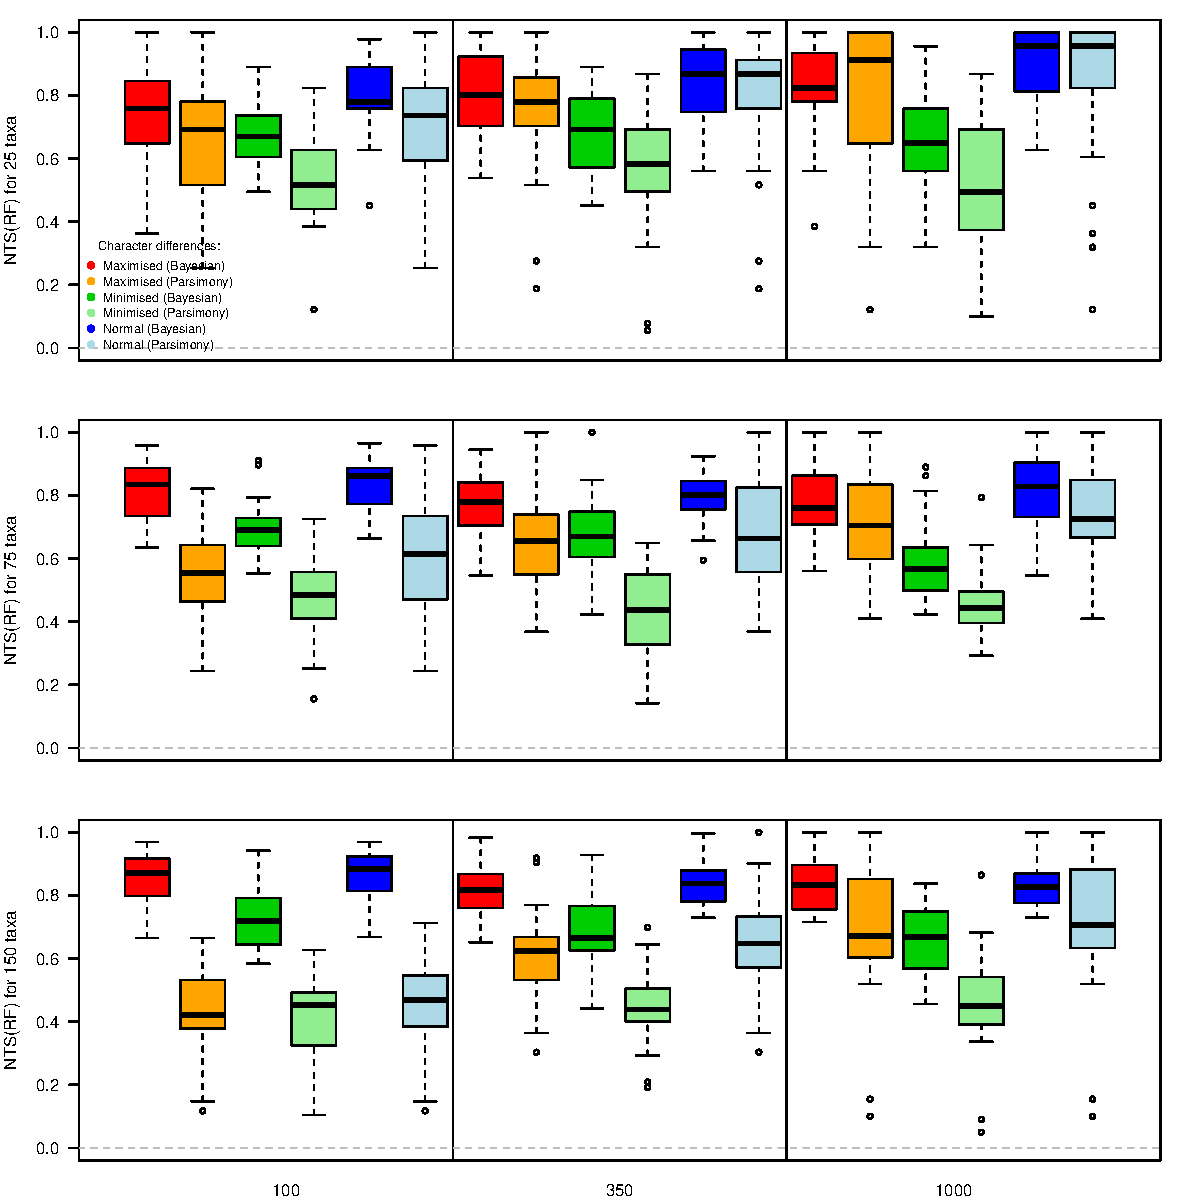
\includegraphics[width=1\textwidth]{../Figures/RF_results_null.pdf} %TG: These figures will be cleaned up once I have the final results.
\caption{Effect of Character Difference on recovering the ``random'' topology. The y axis represents the Normalised Tree Similarity using Robinson-Fould distance for matrices with 25, 75 and 150 taxa from top to bottom respectively. The x axis represents the different Character Difference scenarios and tree inference method with the Maximised Character Difference in Bayesian (red) and under Maximum Parsimony (orange), the Minimised Character Difference in Bayesian (dark green) and under Maximum Parsimony (light green) and the Randomised Character Difference in Bayesian (dark blue) and under Maximum Parsimony (light blue) for matrices of 100, 350 and 1000 characters in the panels from left to right.}
\label{Fig:RF_results_rand}
\end{figure}


\begin{figure}[!htbp]
\centering
   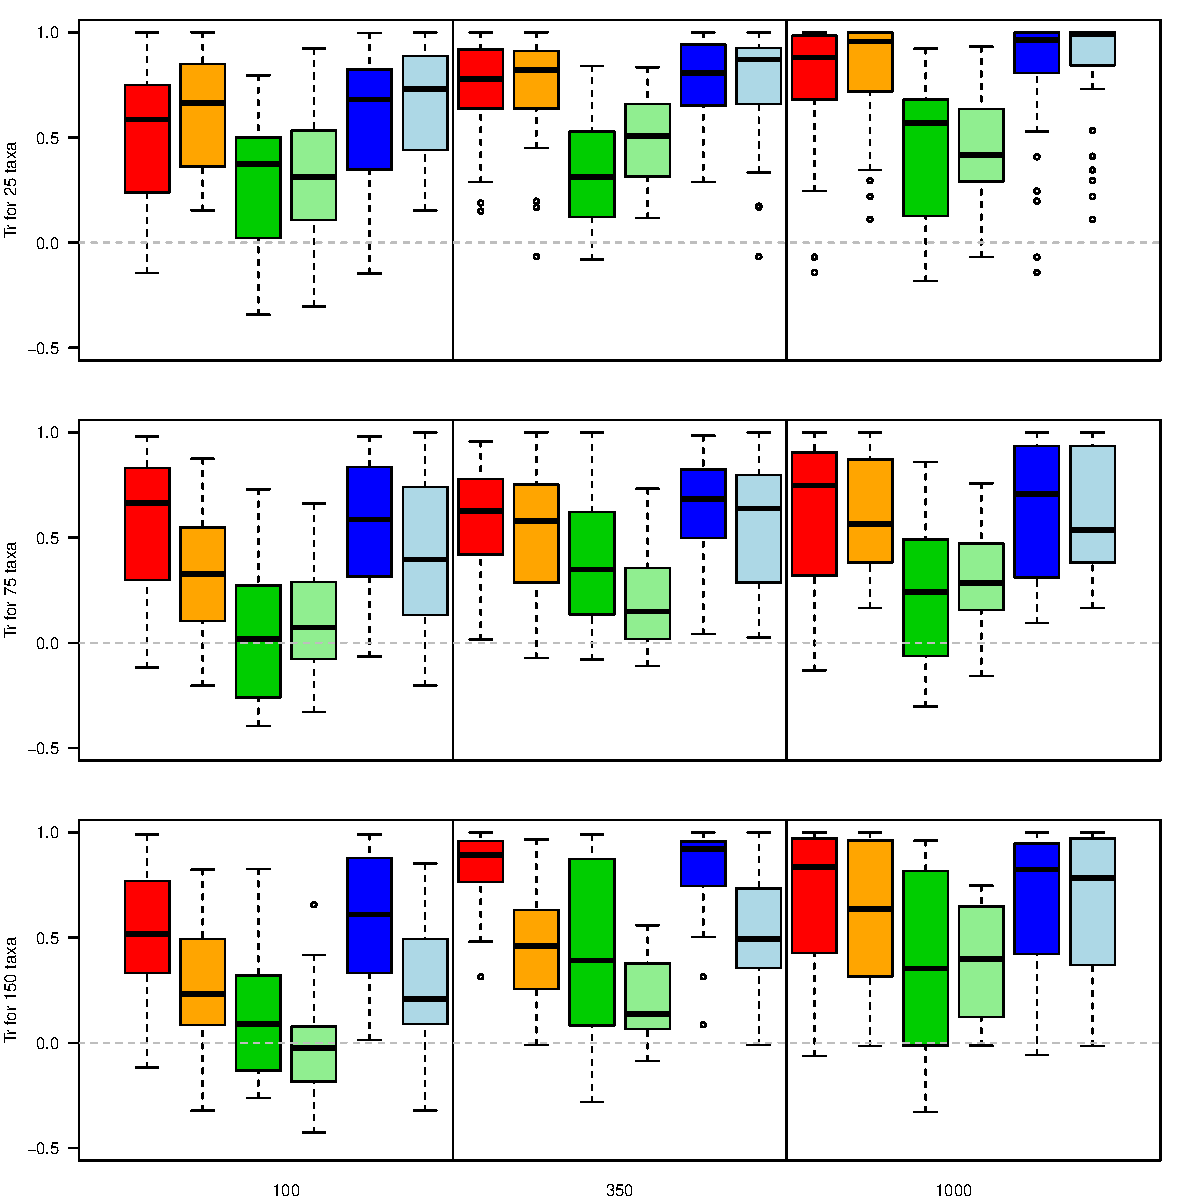
\includegraphics[width=1\textwidth]{../Figures/Tr_results_null.pdf} %TG: These figures will be cleaned up once I have the final results.
\caption{Effect of Character Difference on recovering the ``random'' topology. The axis are identical to figure \ref{Fig:RF_results_rand} but y axis represents the Normalised Tree Similarity using Triplets distance.}
\label{Fig:Tr_results_rand}
\end{figure}


\section{Linear models for anova results}

\subsection{Pooled distributions}

\subsection{Combined distributions}


\section{Distributions summary statistics}

\subsection{Pooled distributions}

\subsection{Combined distributions}



\end{document}